\documentclass[11pt,a4paper]{report}
\usepackage[textwidth=37em,vmargin=30mm]{geometry}
\usepackage{calc,xunicode,amsmath,amssymb,paralist,enumitem,tabu,booktabs,datetime2,xeCJK,xeCJKfntef,listings}
\usepackage{tocloft,fancyhdr,tcolorbox,xcolor,graphicx,eso-pic,xltxtra,xelatexemoji}

\newcommand{\envyear}[0]{2025}
\newcommand{\envdatestr}[0]{2025-06-26}
\newcommand{\envfinaldir}[0]{webdb/2025/20250626/final}

\usepackage[hidelinks]{hyperref}
\hypersetup{
    colorlinks=false,
    pdfpagemode=FullScreen,
    pdftitle={Web Digest - \envdatestr}
}

\setlength{\cftbeforechapskip}{10pt}
\renewcommand{\cftchapfont}{\rmfamily\bfseries\large\raggedright}
\setlength{\cftbeforesecskip}{2pt}
\renewcommand{\cftsecfont}{\sffamily\small\raggedright}

\setdefaultleftmargin{2em}{2em}{1em}{1em}{1em}{1em}

\usepackage{xeCJK,xeCJKfntef}
\xeCJKsetup{PunctStyle=plain,RubberPunctSkip=false,CJKglue=\strut\hskip 0pt plus 0.1em minus 0.05em,CJKecglue=\strut\hskip 0.22em plus 0.2em}
\XeTeXlinebreaklocale "zh"
\XeTeXlinebreakskip = 0pt


\setmainfont{Brygada 1918}
\setromanfont{Brygada 1918}
\setsansfont{IBM Plex Sans}
\setmonofont{JetBrains Mono NL}
\setCJKmainfont{Noto Serif CJK SC}
\setCJKromanfont{Noto Serif CJK SC}
\setCJKsansfont{Noto Sans CJK SC}
\setCJKmonofont{Noto Sans CJK SC}

\setlength{\parindent}{0pt}
\setlength{\parskip}{8pt}
\linespread{1.15}

\lstset{
	basicstyle=\ttfamily\footnotesize,
	numbersep=5pt,
	backgroundcolor=\color{black!5},
	showspaces=false,
	showstringspaces=false,
	showtabs=false,
	tabsize=2,
	captionpos=b,
	breaklines=true,
	breakatwhitespace=true,
	breakautoindent=true,
	linewidth=\textwidth
}






\newcommand{\coverpic}[2]{
    % argv: itemurl, authorname
    Cover photo by #2~~(\href{#1}{#1})
}
\newcommand{\makeheader}[0]{
    \begin{titlepage}
        % \newgeometry{hmargin=15mm,tmargin=21mm,bmargin=12mm}
        \begin{center}
            
            \rmfamily\scshape
            \fontspec{BaskervilleF}
            \fontspec{Old Standard}
            \fontsize{59pt}{70pt}\selectfont
            WEB\hfill DIGEST
            
            \vfill
            % \vskip 30pt
            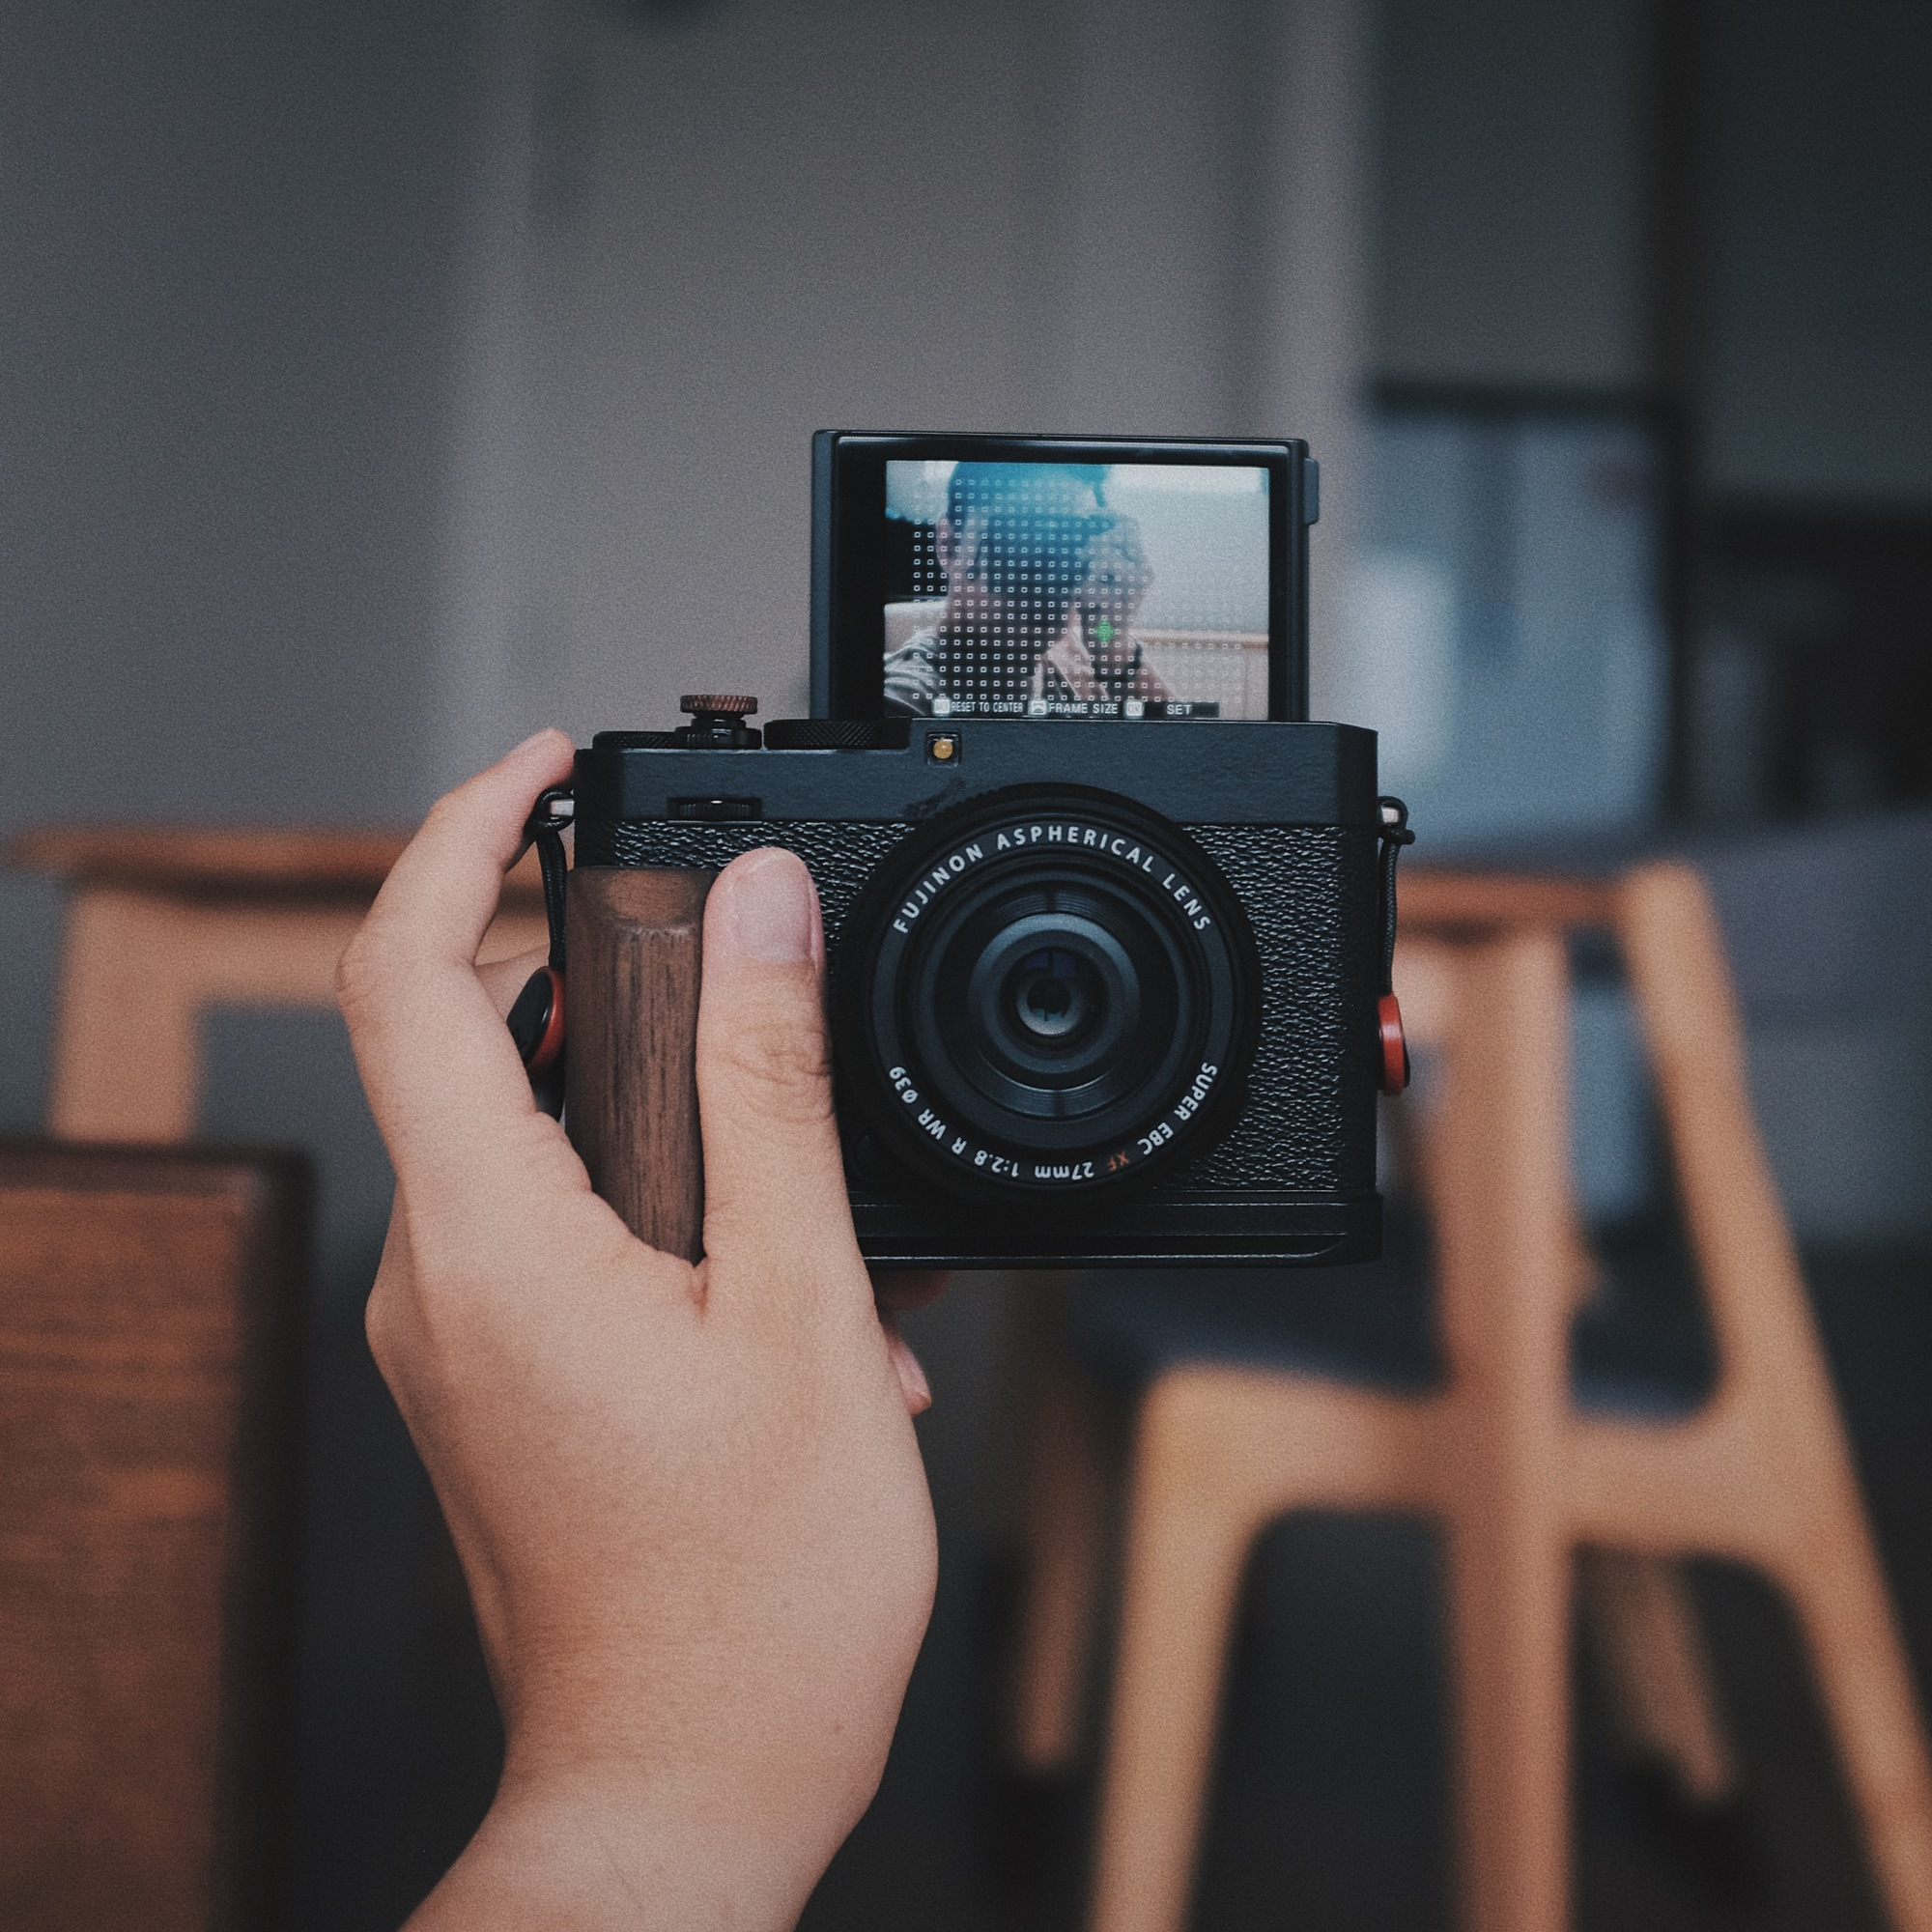
\includegraphics[width=\linewidth]{\envfinaldir/coverpic-prod.jpg}\par
            % \vskip 30pt
            \vfill

            \normalsize\rmfamily\scshape
            \copyright{} The Web Digest Project \hfill\large \envdatestr
        \end{center}
    \end{titlepage}
    % \restoregeometry
}
\newcommand{\simplehref}[1]{%
    \textcolor{blue!80!green}{\href{#1}{#1}}%
}
\renewcommand{\contentsname}{\center\Huge\sffamily\bfseries Contents\par\vskip 20pt}
\newcounter{ipartcounter}
\setcounter{ipartcounter}{0}
\newcommand{\ipart}[1]{
    % \vskip 20pt
    \clearpage
    \stepcounter{ipartcounter}
    \phantomsection
    \addcontentsline{toc}{chapter}{#1}
    % \begin{center}
    %     \Huge
    %     \sffamily\bfseries
    %     #1
    % \end{center}
    % \vskip 20pt plus 7pt
}
\newcounter{ichaptercounter}
\setcounter{ichaptercounter}{0}
\newcommand{\ichapter}[1]{
    % \vskip 20pt
    \clearpage
    \stepcounter{ichaptercounter}
    \phantomsection
    \addcontentsline{toc}{section}{\numberline{\arabic{ichaptercounter}}#1}
    \begin{center}
        \Huge
        \sffamily\bfseries
        #1
    \end{center}
    \vskip 20pt plus 7pt
}
\newcommand{\entrytitlefont}[1]{\subsection*{\raggedright\Large\sffamily\bfseries#1}}
\newcommand{\entryitemGeneric}[2]{
    % argv: title, url
    \parbox{\linewidth}{
        \entrytitlefont{#1}\par\vskip 5pt
        \footnotesize\ttfamily\mdseries
        \simplehref{#2}
    }\vskip 11pt plus 11pt minus 1pt
}
\newcommand{\entryitemGithub}[3]{
    % argv: title, url, desc
    \parbox{\linewidth}{
        \entrytitlefont{#1}\par\vskip 5pt
        \footnotesize\ttfamily\mdseries
        \simplehref{#2}\par\vskip 5pt
        \small\rmfamily\mdseries#3
    }\vskip 11pt plus 11pt minus 1pt
}
\newcommand{\entryitemAp}[3]{
    % argv: title, url, desc
    \parbox{\linewidth}{
        \entrytitlefont{#1}\par\vskip 5pt
        \footnotesize\ttfamily\mdseries
        \simplehref{#2}\par\vskip 5pt
        \small\rmfamily\mdseries#3
    }\vskip 11pt plus 11pt minus 1pt
}
\newcommand{\entryitemHackernews}[3]{
    % argv: title, hnurl, rawurl
    % \parbox{\linewidth}{
    %     \entrytitlefont{#1}\par\vskip 5pt
    %     \footnotesize\ttfamily\mdseries
    %     \simplehref{#3}\par
    %     \textcolor{black!50}{\href{#2}{#2}}
    % }\vskip 11pt plus 11pt minus 1pt
    \begin{minipage}{\linewidth}
            \entrytitlefont{#1}\par\vskip 5pt
            \footnotesize\ttfamily\mdseries
            \simplehref{#3}\par
            \textcolor{black!50}{\href{#2}{#2}}
    \end{minipage}\par\vskip 11pt plus 11pt minus 1pt
}







\begin{document}

\makeheader

\tableofcontents\clearpage




\ipart{Developers}
\ichapter{Hacker News}
\entryitemTwoLinks{A new pyramid-like shape always lands the same side up}{https://news.ycombinator.com/item?id=44381297}{https://www.quantamagazine.org/a-new-pyramid-like-shape-always-lands-the-same-side-up-20250625/}

\entryitemTwoLinks{-2000 Lines of code}{https://news.ycombinator.com/item?id=44381252}{https://www.folklore.org/Negative\_2000\_Lines\_Of\_Code.html}

\entryitemTwoLinks{Games run faster on SteamOS than Windows 11, Ars testing finds}{https://news.ycombinator.com/item?id=44381144}{https://arstechnica.com/gaming/2025/06/games-run-faster-on-steamos-than-windows-11-ars-testing-finds/}

\entryitemTwoLinks{Libxml2's "no security embargoes" policy}{https://news.ycombinator.com/item?id=44381093}{https://lwn.net/SubscriberLink/1025971/73f269ad3695186d/}

\entryitemTwoLinks{LM Studio is now an MCP Host}{https://news.ycombinator.com/item?id=44379792}{https://lmstudio.ai/blog/lmstudio-v0.3.17}

\entryitemTwoLinks{Build and Host AI-Powered Apps with Claude – No Deployment Needed}{https://news.ycombinator.com/item?id=44379673}{https://www.anthropic.com/news/claude-powered-artifacts}

\entryitemTwoLinks{What Problems to Solve (1966)}{https://news.ycombinator.com/item?id=44379606}{http://genius.cat-v.org/richard-feynman/writtings/letters/problems}

\entryitemTwoLinks{Iroh: A library to establish direct connection between peers}{https://news.ycombinator.com/item?id=44379173}{https://github.com/n0-computer/iroh}

\entryitemTwoLinks{Getting ready to issue IP address certificates}{https://news.ycombinator.com/item?id=44379034}{https://community.letsencrypt.org/t/getting-ready-to-issue-ip-address-certificates/238777}

\entryitemTwoLinks{Foreign Scammers Use U.S. Banks to Fleece Americans}{https://news.ycombinator.com/item?id=44377104}{https://www.propublica.org/article/pig-butchering-scam-cybercrime-us-banks-money-laundering}

\entryitemTwoLinks{OpenAI charges by the minute, so speed up your audio}{https://news.ycombinator.com/item?id=44376989}{https://george.mand.is/2025/06/openai-charges-by-the-minute-so-make-the-minutes-shorter/}

\entryitemTwoLinks{Second study finds Uber used opaque algorithm to dramatically boost profits}{https://news.ycombinator.com/item?id=44376928}{https://www.theguardian.com/technology/2025/jun/25/second-study-finds-uber-used-opaque-algorithm-to-dramatically-boost-profits}

\entryitemTwoLinks{Gemini CLI}{https://news.ycombinator.com/item?id=44376919}{https://blog.google/technology/developers/introducing-gemini-cli-open-source-ai-agent/}

\entryitemTwoLinks{Third places and neighborhood entrepreneurship (2024)}{https://news.ycombinator.com/item?id=44376362}{https://www.nber.org/papers/w32604}

\entryitemTwoLinks{Show HN: Scream to Unlock – Blocks social media until you scream ``I'm a loser''}{https://news.ycombinator.com/item?id=44375761}{https://news.ycombinator.com/item?id=44375761}

\entryitemTwoLinks{The Fairphone (Gen. 6)}{https://news.ycombinator.com/item?id=44375451}{https://shop.fairphone.com/the-fairphone-gen-6}

\entryitemTwoLinks{Lyon Drops Microsoft to Boost Digital Sovereignty}{https://news.ycombinator.com/item?id=44375121}{https://digitrendz.blog/newswire/business/19813/lyon-drops-microsoft-office-to-boost-digital-sovereignty/}

\entryitemTwoLinks{Reading NFC Passport Chips in Linux}{https://news.ycombinator.com/item?id=44374574}{https://shkspr.mobi/blog/2025/06/reading-nfc-passport-chips-in-linux/}

\entryitemTwoLinks{How renewables are saving Texans billions}{https://news.ycombinator.com/item?id=44373524}{https://www.theclimatebrink.com/p/how-renewables-are-saving-texans}

\entryitemTwoLinks{A new PNG spec}{https://news.ycombinator.com/item?id=44373504}{https://www.programmax.net/articles/png-is-back/}


\ipart{Developers~~~~(zh-Hans)}
\ichapter{Solidot}
\entryitemGeneric{\hskip 0pt{}Anker 等公司召回的移动电源使用了安普瑞斯的电芯 }{https://www.solidot.org/story?sid=81644}

\entryitemGeneric{\hskip 0pt{}微软向 Windows 10 用户提供扩展安全更新}{https://www.solidot.org/story?sid=81643}

\entryitemGeneric{\hskip 0pt{}阳光为什么能高效的蒸发水}{https://www.solidot.org/story?sid=81642}

\entryitemGeneric{\hskip 0pt{}美国众议院禁止工作人员使用 WhatsApp}{https://www.solidot.org/story?sid=81641}

\entryitemGeneric{\hskip 0pt{}Fedora 讨论放弃支持 32 位包}{https://www.solidot.org/story?sid=81640}

\entryitemGeneric{\hskip 0pt{}中国五月份太阳能装机容量创下新记录}{https://www.solidot.org/story?sid=81639}

\entryitemGeneric{\hskip 0pt{}Vera C. Rubin 天文台公布了首批宇宙全景照}{https://www.solidot.org/story?sid=81638}

\entryitemGeneric{\hskip 0pt{}Google Chromebook 笔记本电脑集成 AI 功能}{https://www.solidot.org/story?sid=81637}

\entryitemGeneric{\hskip 0pt{}亚马逊加速发射互联网宽带卫星}{https://www.solidot.org/story?sid=81636}

\entryitemGeneric{\hskip 0pt{}IYO 就 IO 商标起诉 OpenAI}{https://www.solidot.org/story?sid=81635}

\entryitemGeneric{\hskip 0pt{}Firefox 140 释出}{https://www.solidot.org/story?sid=81634}

\entryitemGeneric{\hskip 0pt{}玻璃瓶瓶盖显著增加了饮料中的微塑料含量}{https://www.solidot.org/story?sid=81633}

\entryitemGeneric{\hskip 0pt{}博士数量超过学界需求}{https://www.solidot.org/story?sid=81632}

\entryitemGeneric{\hskip 0pt{}马斯克现身YC大会:谈``智能大爆炸''时代的生存法则,结合PayPal、SpaceX、特斯拉、xAI创业史,详解如何使用第一性原理}{https://www.solidot.org/story?sid=81631}

\entryitemGeneric{\hskip 0pt{}微软设定 Windows 11 系统还原点的有效时间为 60 天}{https://www.solidot.org/story?sid=81630}

\entryitemGeneric{\hskip 0pt{}一颗死亡的 NASA 卫星突然发射出强大的射电信号}{https://www.solidot.org/story?sid=81629}

\entryitemGeneric{\hskip 0pt{}分析师认为 AI 没有做好它的工作}{https://www.solidot.org/story?sid=81628}

\entryitemGeneric{\hskip 0pt{}减肥显著提升一个人的自尊水平}{https://www.solidot.org/story?sid=81627}

\entryitemGeneric{\hskip 0pt{}AI 如何影响印度的呼叫中心行业}{https://www.solidot.org/story?sid=81626}

\entryitemGeneric{\hskip 0pt{}Bill Gates 和 Linus Torvalds 首次同框}{https://www.solidot.org/story?sid=81625}\ichapter{V2EX}
\entryitemGeneric{\hskip 0pt{}[问与答] 🛠️ VMware Tools 同步神器 🚀|一键拉取最新官方版本 📦}{https://www.v2ex.com/t/1141090}

\entryitemGeneric{\hskip 0pt{}[问与答] macOS 自带的密码管理器,为啥隔段时间就要输入验证码?}{https://www.v2ex.com/t/1141089}

\entryitemGeneric{\hskip 0pt{}[电影] 寻找一部很早以前出的关于 ai 的电影(电视剧?)}{https://www.v2ex.com/t/1141088}

\entryitemGeneric{\hskip 0pt{}[分享创造] REM - 基于 Rclone 的文件管理器}{https://www.v2ex.com/t/1141087}

\entryitemGeneric{\hskip 0pt{}[分享创造] 做了个找保姆的平台--找个保姆,解决了我妈找保姆被坑的问题}{https://www.v2ex.com/t/1141085}

\entryitemGeneric{\hskip 0pt{}[MacBook Pro] 京东国补+教育优惠¥11749 入手 14 寸 MacBook Pro M4 24+512}{https://www.v2ex.com/t/1141084}

\entryitemGeneric{\hskip 0pt{}[DNS] powerdns-dnsdist 基于域名分流实现}{https://www.v2ex.com/t/1141083}

\entryitemGeneric{\hskip 0pt{}[酷工作] 上海: AIML Engineer,与第三方签合同,首签三年,外资公司 onsite。}{https://www.v2ex.com/t/1141082}

\entryitemGeneric{\hskip 0pt{}[VXNA] 申请收录个人博客: YFZZ Blog(yfzz.net)}{https://www.v2ex.com/t/1141081}

\entryitemGeneric{\hskip 0pt{}[macOS] 手撸编辑器可行吗?}{https://www.v2ex.com/t/1141080}

\entryitemGeneric{\hskip 0pt{}[VXNA] 申请收录 tinyedi.com}{https://www.v2ex.com/t/1141079}

\entryitemGeneric{\hskip 0pt{}[业界八卦] 罗永浩被梁文锋建议「靠嘴吃饭」: ``天赋堪称全国顶尖''}{https://www.v2ex.com/t/1141078}

\entryitemGeneric{\hskip 0pt{}[程序员] gemini-cli 可以使用了}{https://www.v2ex.com/t/1141077}

\entryitemGeneric{\hskip 0pt{}[装修] 小米 ap 可以安装在吊顶上吗?}{https://www.v2ex.com/t/1141076}

\entryitemGeneric{\hskip 0pt{}[宽带症候群] 上海电信限速升级?}{https://www.v2ex.com/t/1141075}

\entryitemGeneric{\hskip 0pt{}[Apple] MacBook pro 合盖放家里,晚上回来打开剩余电量 20\%,而且还特别热,这是发生了什么,已经连续 3 天了}{https://www.v2ex.com/t/1141072}

\entryitemGeneric{\hskip 0pt{}[VXNA] 申请收录个人博客 xkhm.net}{https://www.v2ex.com/t/1141071}

\entryitemGeneric{\hskip 0pt{}[OpenAI] Gemini CLI: Google 推出的开源命令行 Agent(预览期间大量免费额度)}{https://www.v2ex.com/t/1141070}

\entryitemGeneric{\hskip 0pt{}[分享发现] https://github.com/google-gemini/gemini-cli}{https://www.v2ex.com/t/1141069}

\entryitemGeneric{\hskip 0pt{}[程序员] 4090 GPU 算力型服务器哪位小伙伴需要?}{https://www.v2ex.com/t/1141068}

\entryitemGeneric{\hskip 0pt{}[iPhone] vivo 是怎么做到读到 iPhone 的短信、推送、电话的?}{https://www.v2ex.com/t/1141067}

\entryitemGeneric{\hskip 0pt{}[Flutter] 请教: flutter 或 Android 更新、热更新方案}{https://www.v2ex.com/t/1141066}

\entryitemGeneric{\hskip 0pt{}[Go 编程语言] XGo 大家用过吗? Golang 加强版}{https://www.v2ex.com/t/1141065}

\entryitemGeneric{\hskip 0pt{}[远程工作] [外企远程] 资深 Java 开发工程师 Senior Java Developer(contractor)}{https://www.v2ex.com/t/1141064}

\entryitemGeneric{\hskip 0pt{}[数据库] sql 占位符替换 TUI 工具}{https://www.v2ex.com/t/1141063}

\entryitemGeneric{\hskip 0pt{}[问与答] 请教一下各位见多识广的 v 友,有没有这么一种远程控制脚本?}{https://www.v2ex.com/t/1141062}

\entryitemGeneric{\hskip 0pt{}[Java] SpringCloudGateway 已经支持了接口的限流和熔断降级,那么还需要在业务层接口做熔断降级限流处理吗?}{https://www.v2ex.com/t/1141061}

\entryitemGeneric{\hskip 0pt{}[教育] 四川高考 - 547 分 - 68000 名次左右选什么专业和学校?}{https://www.v2ex.com/t/1141060}

\entryitemGeneric{\hskip 0pt{}[分享创造] Vibe 了一个 \_代码质量可能很高\_ 脚手架, Gemini 给出的项目质量评估是 9.5/10...}{https://www.v2ex.com/t/1141058}

\entryitemGeneric{\hskip 0pt{}[分享创造] AI 能帮你自动化排版了?我开发的这款微信 Markdown 编辑器全面支持 API 和 MCP 能力}{https://www.v2ex.com/t/1141057}

\entryitemGeneric{\hskip 0pt{}[分享创造] 做了个多语言的 HEIC 转 JPG 的网站}{https://www.v2ex.com/t/1141055}

\entryitemGeneric{\hskip 0pt{}[教育] 高考成绩下来了,请教一下老前辈们的意见}{https://www.v2ex.com/t/1141053}

\entryitemGeneric{\hskip 0pt{}[宽带症候群] 发现北京联通已经禁止 CUAdmin 登录了}{https://www.v2ex.com/t/1141052}

\entryitemGeneric{\hskip 0pt{}[分享创造] LLM 解读最新\&最热的 arXiv 论文,每天 700+篇,想了解 AI 领域最新进展的朋友不要错过哈~~}{https://www.v2ex.com/t/1141050}

\entryitemGeneric{\hskip 0pt{}[新手求助] 一个认识一个月财产谈崩的帖子为啥要置顶?}{https://www.v2ex.com/t/1141049}

\entryitemGeneric{\hskip 0pt{}[宽带症候群] 成都奠信访问成都镰通,绕路北京,限速 500KB/S,有解决方案吗?}{https://www.v2ex.com/t/1141047}

\entryitemGeneric{\hskip 0pt{}[宽带症候群] 延期了 3 年的事,这一周全部干完了,把家庭网络重新梳理了一遍}{https://www.v2ex.com/t/1141046}

\entryitemGeneric{\hskip 0pt{}[生活] 一个希望 V2 上的女网友参与评论的帖子}{https://www.v2ex.com/t/1141045}

\entryitemGeneric{\hskip 0pt{}[教育] 各位彦祖,亦菲 老弟高考 527 物化生 求推荐学校和专业}{https://www.v2ex.com/t/1141044}

\entryitemGeneric{\hskip 0pt{}[Android] android studio 安装之后缺少预置模块模板是什么情况}{https://www.v2ex.com/t/1141042}

\entryitemGeneric{\hskip 0pt{}[问与答] 为了讨好领导,浪费资源,小伙伴们你们怎么看?}{https://www.v2ex.com/t/1141041}

\entryitemGeneric{\hskip 0pt{}[问与答] 请问 5 匹空调哪个品牌性价高?}{https://www.v2ex.com/t/1141040}

\entryitemGeneric{\hskip 0pt{}[程序员] 想做一个简单的知识库 AI,最基本的问答+检索知识库的能力给客户用,不知道目前最优方案是什么?}{https://www.v2ex.com/t/1141039}

\entryitemGeneric{\hskip 0pt{}[宽带症候群] Windows 系统下 Clash.Meta 第三方代理软件问题}{https://www.v2ex.com/t/1141038}

\entryitemGeneric{\hskip 0pt{}[酷工作] [郑州] 招聘 产品经理 1 名-自研-双休弹性-五险一金}{https://www.v2ex.com/t/1141037}

\entryitemGeneric{\hskip 0pt{}[问与答] 现在我有三个场景用到大模型,但是不知道该怎么选,用的比较少,希望有大佬可以推荐下。}{https://www.v2ex.com/t/1141036}

\entryitemGeneric{\hskip 0pt{}[VPS] 🔥 [lll.host] 新加坡传家宝 · 4 核 4G 火爆开售🔥}{https://www.v2ex.com/t/1141035}

\entryitemGeneric{\hskip 0pt{}[问与答] 各位佬有什么副业可以做}{https://www.v2ex.com/t/1141034}

\entryitemGeneric{\hskip 0pt{}[问与答] 代理的 HTTPS 解密你们开了吗,有什么安全的去广告脚本}{https://www.v2ex.com/t/1141032}

\entryitemGeneric{\hskip 0pt{}[Apple] 小心翼翼的问个苹果笔电企业机升级 macOS26 问题}{https://www.v2ex.com/t/1141031}


\ipart{Generic News}







\clearpage
\leavevmode\vfill
\footnotesize

Copyright \copyright{} 2023-2025 Neruthes and other contributors.

This document is published with CC BY-NC-ND 4.0 license.

The entries listed in this newsletter may be copyrighted by their respective creators.

This newsletter is generated by the Web Digest project.

The newsletters are also delivered via Telegram channel \CJKunderline{\href{https://t.me/webdigestchannel}{https://t.me/webdigestchannel}}.\\
RSS feed is available at \CJKunderline{\href{https://webdigest.pages.dev/rss.xml}{https://webdigest.pages.dev/rss.xml}}.

This newsletter is available in PDF at
\CJKunderline{\href{https://webdigest.pages.dev/}{https://webdigest.pages.dev/}}.

The source code being used to generate this newsletter is available at\\
\CJKunderline{\href{https://github.com/neruthes/webdigest}{https://github.com/neruthes/webdigest}}.

This newsletter is also available in
\CJKunderline{\href{http://webdigest.pages.dev/readhtml/\envyear/WebDigest-20250626.html}{HTML}} and
\CJKunderline{\href{https://github.com/neruthes/webdigest/blob/master/markdown/\envyear/WebDigest-20250626.md}{Markdown}}.


\coverpic{https://unsplash.com/photos/woman-relaxes-outdoors-with-floral-accents-RNQFLvZaIao}{Martin Baron}


\end{document}
